% =====================================================================
%  Evolve — The Late Evolutionary Layer
%  Preliminaries, formalism, design space and related work
%  Working document (no results). Author: Tom Offermann, ETH Zürich
% =====================================================================
\documentclass[11pt,a4paper]{article}

% ---------- layout & fonts ----------
\usepackage[a4paper,margin=2.4cm]{geometry}
\usepackage[T1]{fontenc}
\usepackage[utf8]{inputenc}
\IfFileExists{lmodern.sty}{\usepackage{lmodern}\usepackage{microtype}}{\usepackage[expansion=false]{microtype}}
\usepackage{parskip}
\usepackage{enumitem}
\setlist{itemsep=2pt,topsep=4pt}

% ---------- math ----------
\usepackage{amsmath,amssymb,amsthm,mathtools,bm}

% ---------- tables, figures, colors ----------
\usepackage{booktabs,tabularx,array,multirow}
\newcolumntype{L}[1]{>{\raggedright\arraybackslash}p{#1}}
\newcolumntype{Y}{>{\raggedright\arraybackslash}X}
\usepackage{xcolor}
\usepackage{graphicx}
\usepackage{caption}
\captionsetup{font=small,labelfont=bf}
\usepackage{tikz}
\usetikzlibrary{positioning,arrows.meta,shapes.geometric,shapes.misc,fit,backgrounds,calc,decorations.pathreplacing,shadows}
\usepackage{pgfplots}
\pgfplotsset{compat=1.18}
\usepgfplotslibrary{groupplots}
\usepackage[most]{tcolorbox}
\usepackage[ruled,vlined,linesnumbered]{algorithm2e}

% ---------- refs ----------
\usepackage[colorlinks=true,linkcolor=blue!50!black,citecolor=green!40!black,urlcolor=blue!60!black]{hyperref}
\usepackage[capitalise,noabbrev]{cleveref}

% ---------- palette ----------
\definecolor{slow}{HTML}{5B7FA6}     % frozen / gradient components
\definecolor{slowbg}{HTML}{E4ECF5}
\definecolor{fast}{HTML}{D9822B}     % evolutionary components
\definecolor{fastbg}{HTML}{FBEBDD}
\definecolor{mem}{HTML}{4E9A6B}      % memory / archive
\definecolor{membg}{HTML}{E2F1E7}
\definecolor{ink}{HTML}{333333}

% ---------- theorem environments ----------
\theoremstyle{definition}
\newtheorem{definition}{Definition}[section]
\newtheorem{example}[definition]{Example}
\theoremstyle{plain}
\newtheorem{proposition}[definition]{Proposition}
\newtheorem{lemma}[definition]{Lemma}
\newtheorem{conjecture}[definition]{Conjecture}
\theoremstyle{remark}
\newtheorem{remark}[definition]{Remark}

\newtcolorbox{keybox}[1][]{colback=fastbg,colframe=fast,boxrule=0.6pt,arc=2pt,left=6pt,right=6pt,top=4pt,bottom=4pt,fonttitle=\bfseries,#1}
\newtcolorbox{slowbox}[1][]{colback=slowbg,colframe=slow,boxrule=0.6pt,arc=2pt,left=6pt,right=6pt,top=4pt,bottom=4pt,fonttitle=\bfseries,#1}

% ---------- notation macros ----------
\newcommand{\R}{\mathbb{R}}
\newcommand{\N}{\mathbb{N}}
\newcommand{\E}{\mathbb{E}}
\IfFileExists{dsfont.sty}{\usepackage{dsfont}\newcommand{\one}{\mathds{1}}}{\newcommand{\one}{\mathbf{1}}}
\newcommand{\ind}[1]{\one\!\left[#1\right]}
\newcommand{\Dist}{\mathcal{D}}
\newcommand{\Ctx}{\mathcal{C}}
\newcommand{\Gen}{\mathcal{G}}          % genome space
\newcommand{\Lib}{\mathcal{E}}          % expert library
\newcommand{\Arch}{\mathcal{M}}         % archive
\newcommand{\RefSet}{\mathcal{R}}          % reference / few-shot set
\newcommand{\norm}[1]{\left\lVert #1 \right\rVert}
\newcommand{\ip}[2]{\left\langle #1, #2 \right\rangle}
\newcommand{\Ham}{\operatorname{Ham}}
\newcommand{\KL}{\operatorname{KL}}
\newcommand{\JS}{\operatorname{JS}}
\newcommand{\sg}{\operatorname{sg}}
\newcommand{\TopK}{\operatorname{TopK}}
\newcommand{\softmax}{\operatorname{softmax}}
\newcommand{\argmax}{\operatorname*{arg\,max}}
\newcommand{\argmin}{\operatorname*{arg\,min}}
\newcommand{\Var}{\operatorname{Var}}
\newcommand{\fast}[1]{\textcolor{fast}{#1}}
\newcommand{\slowc}[1]{\textcolor{slow}{#1}}
\newcommand{\memc}[1]{\textcolor{mem}{#1}}

\title{\textbf{Evolve --- The Late Evolutionary Layer}\\[4pt]
\large Preliminaries, a unified formalism, the design space, and related work\\[2pt]
\normalsize\itshape A working document for organising ideas --- no results}
\author{Tom Offermann\\ \small ETH Zürich, Department of Computer Science\\ \small\texttt{toffermann@ethz.ch}}
\date{Version of \today}

\begin{document}
\maketitle

\begin{keybox}[title={The pitch in one paragraph}]
Today's models are superb function approximators, but they are \emph{frozen}: they do not adapt after deployment, and fine-tuning them overwrites what they knew.
Evolutionary algorithms (EAs) are the opposite: poor at optimising $10^9$ parameters, but excellent at fast, parallel, gradient-free search in \emph{small}, possibly discrete, possibly non-differentiable spaces.
The \emph{late evolutionary layer} combines the two.
All representational capacity lives in \slowc{\textbf{slow}} components (a pretrained backbone, a library of experts, a decoder) that are trained by gradients and then kept fixed.
All adaptation lives in a \fast{\textbf{fast}}, tiny \emph{genome} ($10^1$--$10^5$ numbers or bits) placed \emph{late} in the architecture, searched by an EA.
Placing it late makes the population \emph{separable}: one copy of the backbone, one shared forward pass, and $N$ cheap evaluations of candidate genomes.
Storing one genome per context yields a \memc{\textbf{memory}} (an archive) that cannot forget, and recalling from it makes re-adaptation fast.
This document fixes notation, formalises these claims, maps the design space, and places five concrete instantiations (F1--F5) in the literature.
\end{keybox}

\tableofcontents
\newpage

% =====================================================================
\section{Motivation: slow components, fast genomes}
\label{sec:motivation}
% =====================================================================

A system that deserves the word \emph{adaptive} should (i)~learn continually without catastrophic forgetting, (ii)~keep structured, reusable memory, (iii)~adapt quickly to new situations on the basis of prior experience, and (iv)~be able to change its own structure, not only its weights.
Gradient-trained networks deliver none of these by default: they are trained once, deployed, and frozen, and every fine-tuning step moves all parameters at once.

The central design decision of this document is to \emph{separate time scales}, in the spirit of complementary learning systems (a slow cortex and a fast hippocampus):

\begin{center}
\begin{tabular}{@{}lll@{}}
\toprule
 & \slowc{\textbf{slow system}} & \fast{\textbf{fast system}} \\
\midrule
what & backbone, experts, decoder & genome $g$ (routing, mixing, masks, rules) \\
size & $10^8$--$10^{10}$ parameters & $10^1$--$10^5$ numbers or bits \\
optimiser & gradient descent, pretraining & evolutionary algorithm \\
changes & rarely (or never) & per context, continuously \\
memory & weights & \memc{archive of genomes} \\
\bottomrule
\end{tabular}
\end{center}

\Cref{fig:big-picture} shows the resulting architecture. The rest of this section explains, informally, \emph{why} an EA belongs exactly in the orange box; \cref{sec:layer} makes each point precise.

\begin{figure}[t]
\centering
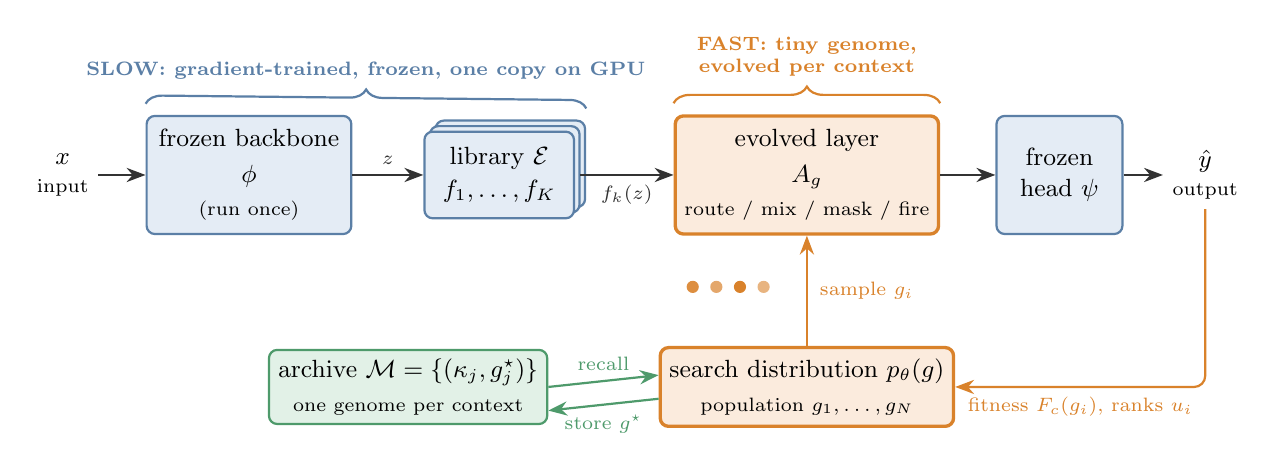
\begin{tikzpicture}[
  font=\small,
  >={Stealth[length=2.4mm]},
  slowblk/.style={draw=slow,fill=slowbg,rounded corners=3pt,thick,minimum height=1.5cm,align=center},
  fastblk/.style={draw=fast,fill=fastbg,rounded corners=3pt,very thick,minimum height=1.5cm,align=center},
  memblk/.style={draw=mem,fill=membg,rounded corners=3pt,thick,align=center},
  lbl/.style={font=\scriptsize\itshape,text=ink!80}
]
% input
\node[align=center] (x) at (0,0) {$x$\\[-1pt]{\scriptsize input}};
% backbone
\node[slowblk,minimum width=2.6cm,right=0.6cm of x] (bb) {frozen backbone\\[2pt]$\phi$\\[1pt]{\scriptsize (run once)}};
% experts stack
\node[slowblk,minimum width=1.9cm,minimum height=1.1cm,right=0.9cm of bb,yshift=4pt,xshift=4pt] (e3) {};
\node[slowblk,minimum width=1.9cm,minimum height=1.1cm,right=0.9cm of bb,yshift=2pt,xshift=2pt] (e2) {};
\node[slowblk,minimum width=1.9cm,minimum height=1.1cm,right=0.9cm of bb] (e1) {library $\Lib$\\[1pt]$f_1,\dots,f_K$};
% evolved layer
\node[fastblk,minimum width=2.7cm,right=1.25cm of e1] (A) {evolved layer\\[2pt]$A_{g}$\\[1pt]{\scriptsize route / mix / mask / fire}};
% head
\node[slowblk,minimum width=1.6cm,right=0.7cm of A] (psi) {frozen\\ head $\psi$};
\node[align=center,right=0.5cm of psi] (y) {$\hat y$\\[-1pt]{\scriptsize output}};
% arrows forward
\draw[->,thick,ink] (x) -- (bb);
\draw[->,thick,ink] (bb) -- node[above,font=\scriptsize]{$z$} (e1);
\draw[->,thick,ink] ($(e1.east)+(0.06,0)$) -- node[below,font=\scriptsize]{$f_k(z)$} (A);
\draw[->,thick,ink] (A) -- (psi);
\draw[->,thick,ink] (psi) -- (y);
% search distribution
\node[fastblk,minimum width=3.3cm,minimum height=1.0cm,below=1.4cm of A] (p) {search distribution $p_\theta(g)$\\[1pt]{\scriptsize population $g_1,\dots,g_N$}};
% population dots
\foreach \i/\c in {-1.2/fast!90,-0.9/fast!70,-0.6/fast!100,-0.3/fast!60}{
  \fill[\c] ($(A.south)+(\i-0.25,-0.65)$) circle (2.2pt);
}
\draw[->,thick,fast] (p.north) -- node[right,font=\scriptsize,xshift=1pt]{sample $g_i$} (A.south);
% fitness feedback
\draw[->,thick,fast,rounded corners=4pt] (y.south) |- node[pos=0.75,below,font=\scriptsize]{fitness $F_c(g_i)$, ranks $u_i$} (p.east);
% archive
\node[memblk,minimum width=3.3cm,minimum height=0.9cm,left=1.4cm of p] (M) {archive $\Arch=\{(\kappa_j,g_j^\star)\}$\\[1pt]{\scriptsize one genome per context}};
\draw[->,thick,mem] (M.east) -- node[above,font=\scriptsize]{recall} ($(p.west)+(0,0.15)$);
\draw[<-,thick,mem] ($(M.east)+(0,-0.3)$) -- node[below,font=\scriptsize]{store $g^\star$} ($(p.west)+(0,-0.15)$);
% braces
\draw[decorate,decoration={brace,amplitude=6pt,raise=4pt},slow,thick] (bb.north west) -- (e3.north east) node[midway,above=10pt,text=slow,font=\scriptsize\bfseries]{SLOW: gradient-trained, frozen, one copy on GPU};
\draw[decorate,decoration={brace,amplitude=6pt,raise=4pt},fast,thick] (A.north west) -- (A.north east) node[midway,above=10pt,text=fast,font=\scriptsize\bfseries,align=center]{FAST: tiny genome,\\ evolved per context};
\end{tikzpicture}
\caption{\textbf{The late evolutionary layer.} Slow components (blue) are trained by gradient descent and then frozen; only one copy is held in memory and its outputs are shared by the whole population. The fast layer (orange) is parameterised by a tiny genome $g$, searched by an EA using any scalar fitness. The archive (green) stores the best genome per context and seeds future searches.}
\label{fig:big-picture}
\end{figure}

\paragraph{Why the EA should be shallow and late (informal).}
\begin{enumerate}[label=(\alph*)]
\item \textbf{Dimension.} Gradient estimates from a population of size $N$ in dimension $n$ carry a signal fraction of $N/(N+n+1)$ (\cref{prop:alignment}). At $n = 10^9$ this is hopeless for any affordable $N$; at $n \le 10^4$ it is excellent. Below $n\approx 10^3$, full-covariance CMA-ES learns the local metric of the problem and is often the best optimiser available at all.
\item \textbf{Adaptation is low-dimensional.} Fine-tuning a pretrained model succeeds in random subspaces of a few hundred to a few thousand dimensions (\emph{intrinsic dimension}, \cref{sec:related}). The \emph{adaptation} problem is small even when the model is not.
\item \textbf{Separability.} If the genome only acts late, everything before it is identical across the population and is computed once (\cref{prop:cost}). The population then costs roughly one forward pass rather than $N$.
\item \textbf{No forgetting in the slow system.} The backbone never moves, so it cannot forget. All task-specific change is a stored genome that can be swapped or rolled back (\cref{prop:zero-forgetting}).
\item \textbf{Hard decisions and non-differentiable objectives.} Routing, masking, thresholding, exact-match accuracy, worst-group accuracy, and episode returns are all non-differentiable. EAs need only a scalar per candidate.
\end{enumerate}

% =====================================================================
\section{Preliminaries and notation}
\label{sec:prelim}
% =====================================================================

\subsection{Notation}

\begin{center}
\small
\begin{tabularx}{\linewidth}{@{}lX@{}}
\toprule
\textbf{Symbol} & \textbf{Meaning} \\
\midrule
$x,\ y$ & input, target (label / answer / action) \\
$c \in \Ctx$,\ $\Dist_c$ & context (task, domain, damage condition) and its data distribution \\
$\phi$,\ $z=\phi(x)\in\R^{d}$ & frozen backbone (\slowc{slow}) and its features \\
$\Lib = \{f_1,\dots,f_K\}$ & library of frozen experts / adapters / skills (\slowc{slow}) \\
$\psi$ & frozen head or decoder (\slowc{slow}) \\
$g \in \Gen$,\ $n=\dim\Gen$ & genome and its dimension (\fast{fast}); $\Gen \subseteq \R^n$ or $\Gen = \Sigma^n$ for a finite alphabet $\Sigma$ \\
$A_g$ & evolved operator (routing, mixing, masking, firing) parameterised by $g$ \\
$\hat y_g(x) = \psi\big(A_g(\phi(x);\Lib)\big)$ & model output under genome $g$ \\
$F_c(g)$ & fitness of $g$ in context $c$ (any scalar) \\
$\RefSet_c$,\ $R=|\RefSet_c|$ & reference (few-shot) set used to estimate $F_c$ \\
$p_\theta(g)$ & search distribution with parameters $\theta$ \\
$N$,\ $g_1,\dots,g_N$ & population size and population \\
$u_i$ & rank-based utility of member $i$ \\
$\sigma$,\ $m$,\ $C$ & ES step size, mean, covariance \\
$\Arch = \{(\kappa_j, g^\star_j, \hat F_j)\}$ & archive: context key, best genome, its fitness (\memc{memory}) \\
$L$,\ $\ell$,\ $\rho = (L-\ell)/L$ & network depth, depth at which the genome acts, suffix fraction \\
$B$,\ $C_{\text{layer}}$,\ $C_A$ & batch size, cost of one layer, cost of the evolved operator \\
\bottomrule
\end{tabularx}
\end{center}

\subsection{The optimisation problem}

For a context $c$ the fast system solves the black-box problem
\begin{equation}
\label{eq:problem}
g^\star_c \in \argmax_{g\in\Gen}\; F_c(g), \qquad F_c(g) = \E_{(x,y)\sim\Dist_c}\big[r\big(\hat y_g(x), y\big)\big] - \beta\,\Omega(g),
\end{equation}
where $r$ is any per-example reward (accuracy, log-likelihood, exact match, return) and $\Omega$ is a regulariser (e.g.\ $\norm{g}_1$ or a KL leash to the unmodified model). In practice $F_c$ is estimated on a reference set $\RefSet_c$:
$\hat F_c(g) = \tfrac{1}{R}\sum_{(x,y)\in\RefSet_c} r(\hat y_g(x), y) - \beta\,\Omega(g)$.
Nothing requires $r$, $A_g$ or $\psi$ to be differentiable.

\subsection{Evolution strategies as search-gradient methods}

Instead of optimising $F$ directly, ES optimises the \emph{expected} fitness under a search distribution,
\begin{equation}
J(\theta) = \E_{g\sim p_\theta}\big[F(g)\big], \qquad
\nabla_\theta J = \E_{g\sim p_\theta}\big[F(g)\,\nabla_\theta \log p_\theta(g)\big],
\end{equation}
the \emph{log-likelihood trick}, estimated by Monte Carlo over the population. For an isotropic Gaussian $p_\theta = \mathcal{N}(m,\sigma^2 I)$ with $g_i = m + \sigma\epsilon_i$ this becomes the familiar
\begin{equation}
\label{eq:es}
\widehat{\nabla_m J} = \frac{1}{N\sigma}\sum_{i=1}^N u_i\,\epsilon_i, \qquad m \leftarrow m + \alpha\,\widehat{\nabla_m J}.
\end{equation}
Three standard variance reductions are used throughout:
\begin{itemize}
\item \textbf{Antithetic sampling:} evaluate $m\pm\sigma\epsilon_i$ and use the difference $\tfrac12\big(F(m+\sigma\epsilon_i)-F(m-\sigma\epsilon_i)\big)$; this cancels the constant and all even-order Taylor terms.
\item \textbf{Rank-based utilities:} replace $F(g_i)$ by $u_i$, a fixed function of its rank. This makes the update invariant to monotone transformations of $F$ (accuracy vs.\ log-likelihood) and robust to outliers.
\item \textbf{Common random numbers (CRN):} all members of a generation are evaluated on the \emph{same} reference batch and the same environment seeds. Without CRN, differences between members are dominated by evaluation noise.
\end{itemize}

\subsection{Natural gradients: one framework for CMA-ES, ES and discrete EDAs}

The \emph{information-geometric optimisation} (IGO) view takes the natural gradient $\tilde\nabla_\theta J = \mathcal{I}(\theta)^{-1}\nabla_\theta J$ (with $\mathcal{I}$ the Fisher information of $p_\theta$), which makes the update independent of how $\theta$ is parameterised:
\begin{equation}
\label{eq:igo}
\theta \leftarrow \theta + \eta \sum_{i=1}^N u_i\,\mathcal{I}(\theta)^{-1}\nabla_\theta\log p_\theta(g_i).
\end{equation}
Different choices of $p_\theta$ recover the algorithms used in this document:

\begin{center}
\small
\begin{tabularx}{\linewidth}{@{}p{2.6cm}p{3.6cm}p{3.3cm}X@{}}
\toprule
genome & $p_\theta$ & algorithm & regime \\
\midrule
continuous, small & $\mathcal{N}(m,\sigma^2 C)$ & CMA-ES & $n\lesssim 10^3$ (full $C$), $\lesssim 10^5$ (diagonal $C$) \\
continuous, matrices & $\mathcal{N}(W,\sigma^2 I)$, low-rank samples & EGGROLL-style ES & up to $10^9$, but see \cref{prop:alignment} \\
discrete & $\prod_j \mathrm{Cat}(\softmax(\theta_j))$ & PBIL / cGA / IGO-categorical & $10^3$--$10^6$ bits or trits \\
\bottomrule
\end{tabularx}
\end{center}

\paragraph{CMA-ES in brief.} Sample $g_i = m + \sigma C^{1/2}\epsilon_i$; rank; with positive weights $w_1\ge\dots\ge w_\mu$ on the best $\mu$ members,
\begin{align}
m &\leftarrow m + c_m \textstyle\sum_{j=1}^{\mu} w_j\,(g_{j:N} - m),\\
C &\leftarrow (1-c_1-c_\mu)\,C + c_1\, p_c p_c^\top + c_\mu \textstyle\sum_{j=1}^\mu w_j\, y_{j:N}\,y_{j:N}^\top, \qquad y_{j:N} = (g_{j:N}-m)/\sigma,
\end{align}
with an evolution path $p_c$ (rank-one update) and a separate path-length control of $\sigma$. CMA-ES learns a metric: correlated parameters receive correlated perturbations.

\paragraph{Categorical IGO (PBIL-like).} For $p_\theta(g_j = v) = \softmax(\theta_j)_v$, \cref{eq:igo} reduces to
\begin{equation}
\label{eq:pbil}
\theta_{j,v} \leftarrow \theta_{j,v} + \eta\sum_{i=1}^N u_i\,\Big(\ind{g_{i,j}=v} - p_\theta(g_j=v)\Big),
\end{equation}
i.e.\ probabilities move towards the values used by good members.

\subsection{Low-rank ES for weight matrices (EGGROLL)}

For a weight matrix $W\in\R^{a\times b}$, a full Gaussian perturbation costs a separate full-rank matmul per member. Low-rank ES perturbs by $E_i = \tfrac{\sigma}{\sqrt r} A_i B_i^\top$ with $A_i\in\R^{a\times r}$, $B_i\in\R^{b\times r}$, so that
\[
(W + E_i)\,u = Wu + \tfrac{\sigma}{\sqrt r}\,A_i\,(B_i^\top u):
\]
the expensive $Wu$ is shared by all members, and each member adds only $O(r(a+b))$. The aggregate update $\sum_i u_i A_iB_i^\top$ is still full rank. This is the \emph{memory-separable} pattern of \cref{def:sep} applied to the whole network; the late layer pushes it to its extreme.

\subsection{Discrete evolutionary algorithms}

\begin{itemize}
\item \textbf{(1+1) EA:} one parent; each position is mutated independently with probability $1/n$ (to a uniformly random \emph{other} symbol); the offspring replaces the parent if it is not worse.
\item \textbf{$(\mu+\lambda)$ GA:} $\mu$ parents create $\lambda$ offspring by uniform crossover and mutation; the best $\mu$ of parents $\cup$ offspring survive.
\item \textbf{Estimation-of-distribution algorithms} (cGA, PBIL, \cref{eq:pbil}): keep a product distribution instead of a population; trivially parallel on GPUs.
\end{itemize}

\subsection{Quality-diversity and archives}

A \emph{quality-diversity} (QD) algorithm returns many good solutions that behave differently. Given a behaviour descriptor $b(g)\in\mathcal{B}$ and a partition of $\mathcal{B}$ into cells, MAP-Elites keeps in each cell the best solution found so far. We will use the same data structure for \emph{memory}: an archive whose cells are \emph{contexts} rather than behaviours (\cref{sec:continual}).

% =====================================================================
\section{The late evolutionary layer}
\label{sec:layer}
% =====================================================================

\subsection{Definition}

\begin{definition}[Late evolutionary layer]
\label{def:layer}
A \emph{late evolutionary layer} is a model of the form
\begin{equation}
\label{eq:model}
\hat y_g(x) \;=\; \slowc{\psi}\Big(\fast{A_g}\big(\,\slowc{h_{\le\ell}}(x);\ \slowc{\Lib}\,\big)\Big),
\end{equation}
where $\slowc{h_{\le \ell}}$ denotes the first $\ell$ of $L$ layers of a frozen network (with $\phi = h_{\le\ell}$ as the backbone), $\slowc{\Lib}$ and $\slowc{\psi}$ are frozen, and only the genome $g$ of the operator $\fast{A_g}$ is optimised, by an EA, with $n = \dim\Gen \ll$ the number of frozen parameters.
The layer is \emph{late} if $\rho = (L-\ell)/L$, the fraction of computation downstream of the genome, is small.
\end{definition}

The operator $A_g$ covers all instantiations in this document:

\begin{center}
\small
\begin{tabularx}{\linewidth}{@{}llX@{}}
\toprule
operator & genome & example \\
\midrule
routing & logit biases $b_\ell\in\R^K$ & $\tilde s_\ell(h) = W_\ell h + b_\ell$, top-$k$ selection of experts (F1) \\
mixing & coefficients $\alpha\in\R^{G\times K}$ & $W' = W + \sum_k \alpha_{\gamma,k} B_kA_k$ over a LoRA library (F2) \\
firing & ternary weights $w_u\in\{-1,0,1\}^d$ & $h_u = \ind{\ip{w_u}{z} > \tau_u}$, decoded by a codebook (F3) \\
selection/blend & descriptor target $d^\star$, gains $\kappa$ & policy $=$ blend of repertoire skills near $d^\star$ (F4) \\
plasticity & rule parameters $\theta$ & $\Delta W = \mathrm{Rule}_\theta(o,z,M)$, genome defines a learner (F5) \\
\bottomrule
\end{tabularx}
\end{center}

\subsection{Two kinds of separability}

\begin{definition}[Separability]
\label{def:sep}
A population evaluation of $g_1,\dots,g_N$ on inputs $x_1,\dots,x_B$ is
\begin{itemize}
\item \textbf{memory-separable} if all members share one copy of the frozen parameters, and each member adds at most $O(n)$ memory;
\item \textbf{compute-separable at depth $\ell$} if the activations $h_{\le\ell}(x_b)$ do not depend on $g$, so they can be computed once and reused by all $N$ members.
\end{itemize}
\end{definition}

Memory separability holds for every design in this document. Compute separability depends on the \emph{task}:

\begin{center}
\small
\begin{tabular}{@{}lcc@{}}
\toprule
setting & memory-sep. & compute-sep. \\
\midrule
classification, multiple-choice scoring (fixed input) & \checkmark & \checkmark \\
test-time adaptation on a fixed batch & \checkmark & \checkmark \\
routing only at scored token positions of a fixed prompt & \checkmark & \checkmark \\
autoregressive generation (generated tokens depend on $g$) & \checkmark & only for the prompt \\
closed-loop control (observations depend on actions) & \checkmark & $\times$ \\
\bottomrule
\end{tabular}
\end{center}

\begin{figure}[t]
\centering
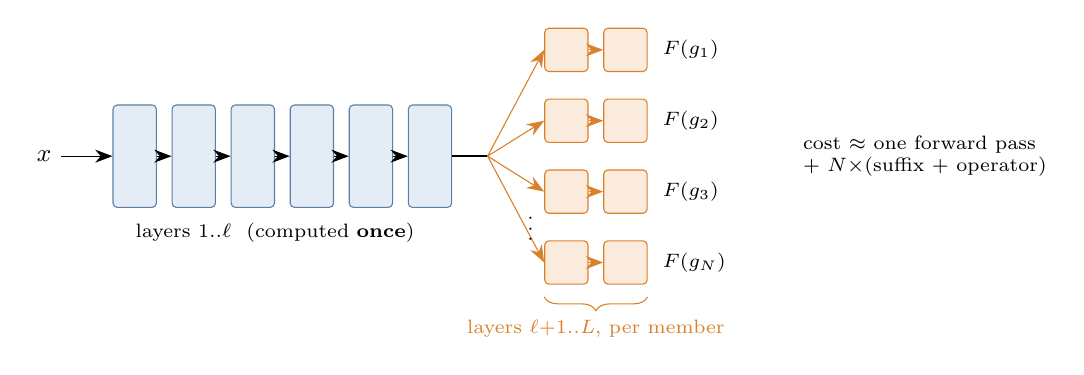
\begin{tikzpicture}[
  font=\small,>={Stealth[length=2.2mm]},
  lay/.style={draw=slow,fill=slowbg,minimum width=0.55cm,minimum height=1.3cm,rounded corners=1.5pt},
  flay/.style={draw=fast,fill=fastbg,minimum width=0.55cm,minimum height=0.55cm,rounded corners=1.5pt},
]
\node (x) at (0,0) {$x$};
\foreach \i in {1,...,6}{ \node[lay] (L\i) at (0.4+0.75*\i,0) {}; }
\node[font=\scriptsize,below=2pt of L3.south east] {layers $1..\ell$ \ (computed \textbf{once})};
\draw[->] (x) -- (L1);
\foreach \i [evaluate=\i as \j using int(\i+1)] in {1,...,5}{ \draw[->] (L\i) -- (L\j); }
\coordinate (split) at ($(L6.east)+(0.45,0)$);
\draw[thick] (L6.east) -- (split);
\foreach \k/\y/\lab in {1/1.35/g_1,2/0.45/g_2,3/-0.45/g_3,4/-1.35/g_N}{
  \node[flay] (A\k) at ($(split)+(1.0,\y)$) {};
  \node[flay] (B\k) at ($(A\k)+(0.75,0)$) {};
  \draw[->,fast] (split) -- (A\k.west);
  \draw[->,fast] (A\k) -- (B\k);
  \node[right=2pt of B\k,font=\scriptsize] (F\k) {$F(\lab)$};
}
\node[font=\scriptsize,rotate=90] at ($(A3)!0.5!(A4)+(-0.45,0)$) {$\cdots$};
\draw[decorate,decoration={brace,amplitude=5pt,mirror,raise=3pt},fast] ($(A4.south west)+(0,-0.05)$) -- ($(B4.south east)+(0,-0.05)$) node[midway,below=8pt,font=\scriptsize,text=fast]{layers $\ell{+}1..L$, per member};
\node[align=left,font=\scriptsize,anchor=west] at ($(F1)+(1.3,-1.35)$) {cost $\approx$ one forward pass\\ $+\ N\times$(suffix $+$ operator)};
\end{tikzpicture}
\caption{\textbf{Compute separability.} If the genome acts only from depth $\ell$ on and the input does not depend on it, the prefix is computed once and fanned out to $N$ members. Only the orange suffix is paid $N$ times.}
\label{fig:fanout}
\end{figure}

\subsection{The cost model}

\begin{proposition}[Speed-up of a late layer]
\label{prop:cost}
Let each of $L$ layers cost $C_{\text{layer}}$ per input, let the operator cost $C_A$ per input and member, and let the genome act from depth $\ell$. For a compute-separable evaluation of $N$ members on $B$ inputs,
\begin{align}
T_{\text{naive}} &= N B\,(L\,C_{\text{layer}} + C_A),\\
T_{\text{sep}} &= B\,\ell\,C_{\text{layer}} + N B\,\big((L-\ell)\,C_{\text{layer}} + C_A\big).
\end{align}
With $\rho = (L-\ell)/L$ and $\kappa = C_A/(L\,C_{\text{layer}})$, the speed-up is
\begin{equation}
\label{eq:speedup}
S \;=\; \frac{T_{\text{naive}}}{T_{\text{sep}}} \;=\; \frac{N(1+\kappa)}{(1-\rho) + N(\rho+\kappa)},
\qquad
\lim_{\rho,\kappa\to0} S = N,
\qquad
\lim_{N\to\infty} S = \frac{1+\kappa}{\rho+\kappa}.
\end{equation}
\end{proposition}
\begin{proof}
Naively, each of the $N$ members runs all $L$ layers and the operator on all $B$ inputs. Under compute separability the first $\ell$ layers are run once per input and the remaining $L-\ell$ layers plus the operator once per member and input. Dividing, and substituting $\ell = (1-\rho)L$ and $C_A = \kappa L C_{\text{layer}}$, gives \cref{eq:speedup}; the limits are immediate.
\end{proof}

\begin{remark}
Two design rules follow. (i)~The speed-up is capped by $1/\rho$: every layer after the genome costs a factor $N$. A frozen decoder $\psi$ behind the evolved layer is only free if it is cheap or cacheable. (ii)~The operator must be cheap compared to a layer ($\kappa \ll \rho$); a mixing operator over $K$ rank-$r$ adapters costs $O(Kr(a+b))$ per token instead of $O(ab)$.
\end{remark}

\begin{figure}[t]
\centering
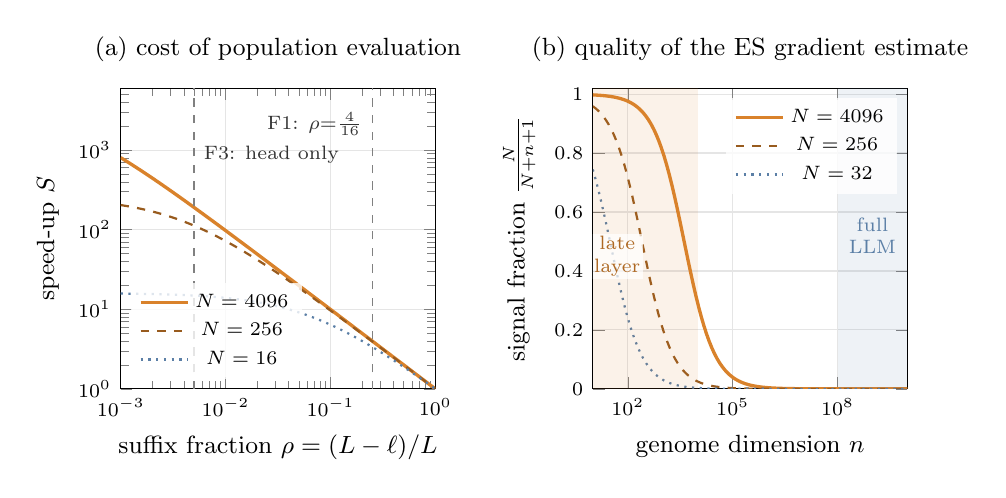
\begin{tikzpicture}
\begin{groupplot}[
  group style={group size=2 by 1,horizontal sep=2.0cm},
  width=0.46\linewidth,height=5.4cm,
  grid=major,grid style={gray!20},
  tick label style={font=\scriptsize},label style={font=\small},
  legend style={font=\scriptsize,draw=none,fill=white,fill opacity=0.8,text opacity=1},
]
\nextgroupplot[
  xmode=log,ymode=log,xmin=1e-3,xmax=1,ymin=1,ymax=6000,
  xlabel={suffix fraction $\rho=(L-\ell)/L$},ylabel={speed-up $S$},
  title={\small (a) cost of population evaluation},
  legend pos=south west,
]
\addplot[fast,very thick,domain=1e-3:1,samples=80] {4096/((1-x)+4096*x)};
\addlegendentry{$N=4096$}
\addplot[fast!70!black,thick,dashed,domain=1e-3:1,samples=80] {256/((1-x)+256*x)};
\addlegendentry{$N=256$}
\addplot[slow,thick,dotted,domain=1e-3:1,samples=80] {16/((1-x)+16*x)};
\addlegendentry{$N=16$}
\draw[gray,dashed] (axis cs:0.25,1) -- (axis cs:0.25,6000) node[pos=0.88,left,font=\scriptsize,text=ink]{F1: $\rho{=}\tfrac{4}{16}$};
\draw[gray,dashed] (axis cs:0.005,1) -- (axis cs:0.005,6000) node[pos=0.78,right,font=\scriptsize,text=ink]{F3: head only};

\nextgroupplot[
  xmode=log,xmin=10,xmax=1e10,ymin=0,ymax=1.02,
  xlabel={genome dimension $n$},ylabel={signal fraction $\frac{N}{N+n+1}$},
  title={\small (b) quality of the ES gradient estimate},
  legend pos=north east,
]
\addplot[fast,very thick,domain=10:1e10,samples=120] {4096/(4096+x+1)};
\addlegendentry{$N=4096$}
\addplot[fast!70!black,thick,dashed,domain=10:1e10,samples=120] {256/(256+x+1)};
\addlegendentry{$N=256$}
\addplot[slow,thick,dotted,domain=10:1e10,samples=120] {32/(32+x+1)};
\addlegendentry{$N=32$}
\fill[fast,opacity=0.10] (axis cs:10,0) rectangle (axis cs:1e4,1.02);
\node[font=\scriptsize,text=fast!80!black,align=center,fill=white,fill opacity=0.7,text opacity=1,inner sep=1pt] at (axis cs:5e1,0.45) {late\\ layer};
\fill[slow,opacity=0.10] (axis cs:1e8,0) rectangle (axis cs:1e10,1.02);
\node[font=\scriptsize,text=slow,align=center] at (axis cs:1e9,0.52) {full\\ LLM};
\end{groupplot}
\end{tikzpicture}
\caption{\textbf{Two reasons to go late and small.} (a)~\Cref{prop:cost} with $\kappa=0$: the speed-up approaches $N$ as the genome moves to the end of the network. (b)~\Cref{prop:alignment}: the fraction of the ES estimate that is signal is $N/(N+n+1)$, excellent for $n\le 10^4$ and negligible at LLM scale.}
\label{fig:cost-dim}
\end{figure}

\subsection{How good is an ES gradient in dimension $n$?}

\begin{proposition}[Signal fraction of the ES estimator]
\label{prop:alignment}
Let $F(g) = \ip{a}{g}$ be locally linear with $a\in\R^n$, and consider the antithetic estimator $\hat\nabla = \frac{1}{2N\sigma}\sum_{i=1}^N \big(F(m+\sigma\epsilon_i) - F(m-\sigma\epsilon_i)\big)\epsilon_i$ with $\epsilon_i\stackrel{\text{iid}}{\sim}\mathcal{N}(0,I_n)$. Then
\begin{equation}
\E\big[\hat\nabla\big] = a, \qquad \E\norm{\hat\nabla}^2 = \norm{a}^2\Big(1+\frac{n+1}{N}\Big),
\qquad
\frac{\norm{\E\hat\nabla}^2}{\E\norm{\hat\nabla}^2} = \frac{N}{N+n+1}.
\end{equation}
In particular, for $n\gg N$ the typical cosine between $\hat\nabla$ and $a$ is $\approx\sqrt{N/n}$.
\end{proposition}
\begin{proof}
For linear $F$, $\tfrac{1}{2\sigma}(F(m+\sigma\epsilon)-F(m-\sigma\epsilon)) = \ip{a}{\epsilon}$, so $\hat\nabla = \frac1N\sum_i X_i$ with $X_i = \epsilon_i\epsilon_i^\top a$ and $\E X_i = a$. Without loss of generality $a = \norm{a}e_1$, so $\E\norm{X_i}^2 = \norm{a}^2\,\E\big[\epsilon_1^2\norm{\epsilon}^2\big] = \norm{a}^2\big(\E\epsilon_1^4 + (n-1)\big) = \norm{a}^2(n+2)$. By independence, $\E\norm{\hat\nabla}^2 = \frac{1}{N}\E\norm{X_1}^2 + \frac{N-1}{N}\norm{a}^2 = \norm{a}^2\big(1+\frac{n+1}{N}\big)$.
\end{proof}

\begin{remark}
This is the quantitative content of ``EAs are slow in high dimensions'': the population must scale with $n$ to keep the estimate informative. A late layer makes $n$ small by design, so the same $N$ that is useless for a full model is near-perfect for the genome.
\end{remark}

\subsection{The design space: where and how big}

\Cref{fig:design-space} places existing work and our instantiations by genome size $n$ and suffix fraction $\rho$. The lower-left region (small $n$, small $\rho$) is where \emph{both} \cref{prop:cost} and \cref{prop:alignment} are favourable. Most existing gradient-free adaptation methods sit at $\rho = 1$ (they perturb inputs or all layers); they are small in $n$ but pay the full forward pass per member.

\begin{figure}[t]
\centering
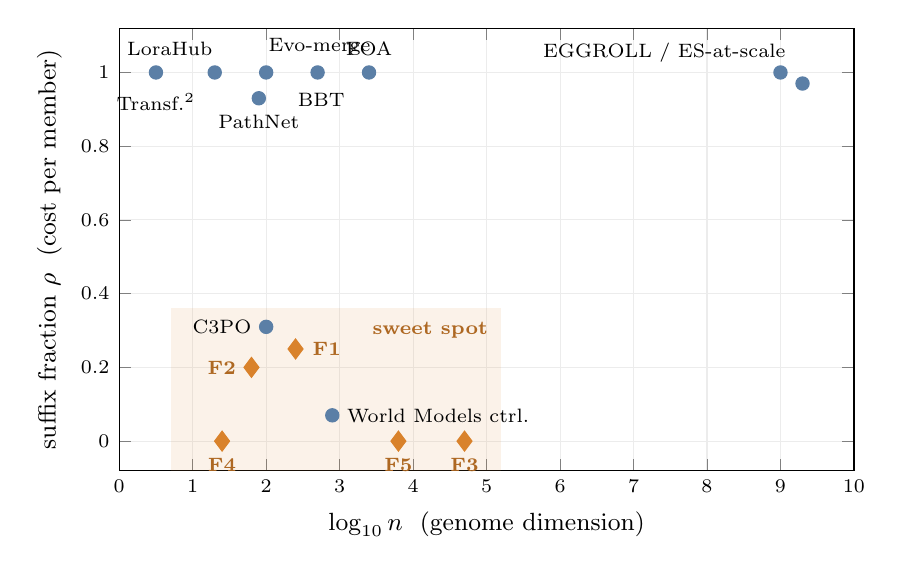
\begin{tikzpicture}
\begin{axis}[
  width=0.9\linewidth,height=7.2cm,
  xmin=0,xmax=10,ymin=-0.08,ymax=1.12,
  xlabel={$\log_{10} n$ \ (genome dimension)},
  ylabel={suffix fraction $\rho$ \ (cost per member)},
  grid=major,grid style={gray!15},
  tick label style={font=\scriptsize},label style={font=\small},
  clip=false,
]
\fill[fast,opacity=0.10] (axis cs:0.7,-0.08) rectangle (axis cs:5.2,0.36);
\node[font=\scriptsize\bfseries,text=fast!80!black,anchor=north east] at (axis cs:5.15,0.35) {sweet spot};
% existing work (blue)
\addplot[only marks,mark=*,mark size=2.4pt,slow] coordinates {
 (9,1) (9.3,0.97) (3.4,1) (2.7,1) (1.3,1) (0.5,1) (2.0,1) (1.9,0.93) (2.0,0.31) (2.9,0.07)};
\node[font=\scriptsize,anchor=south east] at (axis cs:9.2,1.0) {EGGROLL / ES-at-scale};
\node[font=\scriptsize,anchor=south] at (axis cs:3.4,1.02) {FOA};
\node[font=\scriptsize,anchor=north] at (axis cs:2.75,0.97) {BBT};
\node[font=\scriptsize,anchor=south east] at (axis cs:1.4,1.02) {LoraHub};
\node[font=\scriptsize,anchor=north] at (axis cs:0.5,0.97) {Transf.$^2$};
\node[font=\scriptsize,anchor=south west] at (axis cs:1.9,1.02) {Evo-merge};
\node[font=\scriptsize,anchor=north] at (axis cs:1.9,0.91) {PathNet};
\node[font=\scriptsize,anchor=east] at (axis cs:1.93,0.31) {C3PO};
\node[font=\scriptsize,anchor=west] at (axis cs:2.97,0.07) {World Models ctrl.};
% ours (orange)
\addplot[only marks,mark=diamond*,mark size=3.6pt,fast] coordinates {
 (2.4,0.25) (1.8,0.2) (4.7,0.0) (1.4,0.0) (3.8,0.0)};
\node[font=\scriptsize\bfseries,text=fast!80!black,anchor=west] at (axis cs:2.5,0.25) {F1};
\node[font=\scriptsize\bfseries,text=fast!80!black,anchor=east] at (axis cs:1.72,0.2) {F2};
\node[font=\scriptsize\bfseries,text=fast!80!black,anchor=north] at (axis cs:4.7,-0.02) {F3};
\node[font=\scriptsize\bfseries,text=fast!80!black,anchor=north] at (axis cs:1.4,-0.02) {F4};
\node[font=\scriptsize\bfseries,text=fast!80!black,anchor=north] at (axis cs:3.8,-0.02) {F5};
\end{axis}
\end{tikzpicture}
\caption{\textbf{Design space.} Blue: existing gradient-free or evolutionary methods; orange: the instantiations F1--F5 of \cref{sec:instances}. Positions are indicative. Methods at $\rho=1$ pay a full forward pass per candidate; the shaded region is where separability and dimension are both favourable. Closed-loop settings (World Models, F4) are only memory-separable; their $\rho$ refers to the controller's share of computation.}
\label{fig:design-space}
\end{figure}

% =====================================================================
\section{Continual adaptation with a genome archive}
\label{sec:continual}
% =====================================================================

\subsection{Setting}

Contexts arrive as a stream $c_1, c_2,\dots$ (possibly recurring or related). The slow system is fixed. The fast system maintains an archive
\[
\Arch = \big\{(\kappa_j,\ g^\star_j,\ \hat F_j)\big\}_{j},
\]
where $\kappa_j$ is a \emph{key} describing context $j$: for example the mean frozen feature $\bar z = \frac1R\sum_{x\in\RefSet_j}\phi(x)$, or a behavioural descriptor. The archive is a MAP-Elites structure indexed by contexts rather than behaviours.

\begin{algorithm}[h]
\caption{Recall--adapt--store}
\label{alg:recall}
\KwIn{frozen $\phi,\Lib,\psi$; archive $\Arch$; new context $c$ with reference set $\RefSet_c$; budget $T$ generations of $N$ members}
Compute and cache the shared prefix $h_{\le\ell}(x)$ for all $x\in\RefSet_c$\tcp*{once}
$\kappa_c \leftarrow$ key of $c$ (e.g.\ mean prefix feature)\;
\eIf(\tcp*[f]{\memc{recall}}){$\Arch\neq\emptyset$}{
  $\mathcal{Q}\leftarrow$ the $M$ archive genomes with keys nearest to $\kappa_c$\;
  evaluate all of $\mathcal{Q}$ on $\RefSet_c$ \tcp*{one batched population evaluation}
  initialise $p_\theta$ at the best recalled genome, spread from the top recalled genomes\;
}{initialise $p_\theta$ at the identity genome (no modification)}
\For(\tcp*[f]{\fast{adapt}}){$t=1,\dots,T$}{
  sample $g_1,\dots,g_N\sim p_\theta$; evaluate $\hat F_c(g_i)$ with CRN; update $\theta$ by \cref{eq:igo}\;
}
$\Arch\leftarrow\Arch\cup\{(\kappa_c, g^\star_c, \hat F_c(g^\star_c))\}$ \tcp*{\memc{store}}
\Return $g^\star_c$
\end{algorithm}

\subsection{What forgetting means here}

\begin{proposition}[No forgetting by construction]
\label{prop:zero-forgetting}
If the slow system is frozen and, at test time, context $c$ is served with the archived genome $g^\star_c$, then the performance on $c$ after any sequence of later contexts equals the performance at the time $g^\star_c$ was stored.
\end{proposition}
\begin{proof}
$\hat y_{g^\star_c}(x)$ depends only on the frozen $\phi,\Lib,\psi$ and on $g^\star_c$, none of which change after storing.
\end{proof}

The statement is trivial; its value is in isolating the \emph{only two} remaining sources of forgetting:
\begin{enumerate}
\item \textbf{Key mis-recall.} If the context of a test input is unknown, it must be inferred from $\kappa$. Mis-recall rate is directly measurable.
\item \textbf{Interference in shared structure.} If new contexts extend a shared structure (e.g.\ new codewords in a shared decoder, F3), old contexts can be confused with new ones. This is decoding interference, not weight drift.
\end{enumerate}

\subsection{Metrics}

With $A_{t,j}$ the accuracy on context $j$ after learning context $t$, and $T$ contexts:
\begin{align}
\bar A_T &= \frac1T\sum_{j=1}^T A_{T,j} &&\text{(final average accuracy)}\\
\mathrm{BWT} &= \frac{1}{T-1}\sum_{j<T}\big(A_{T,j} - A_{j,j}\big) &&\text{(backward transfer; } < 0 \text{ is forgetting)}\\
\mathrm{AUC}_c(S) &= \frac1S\sum_{s=1}^{S} F_c\big(g^{(s)}_{\text{best}}\big) &&\text{(adaptation speed over the first } S \text{ evaluations)}
\end{align}
$\mathrm{AUC}$ on \emph{revisited} vs.\ \emph{new} contexts is the number that shows whether memory helps. A stream without recurring or related contexts cannot show it.

\begin{figure}[t]
\centering
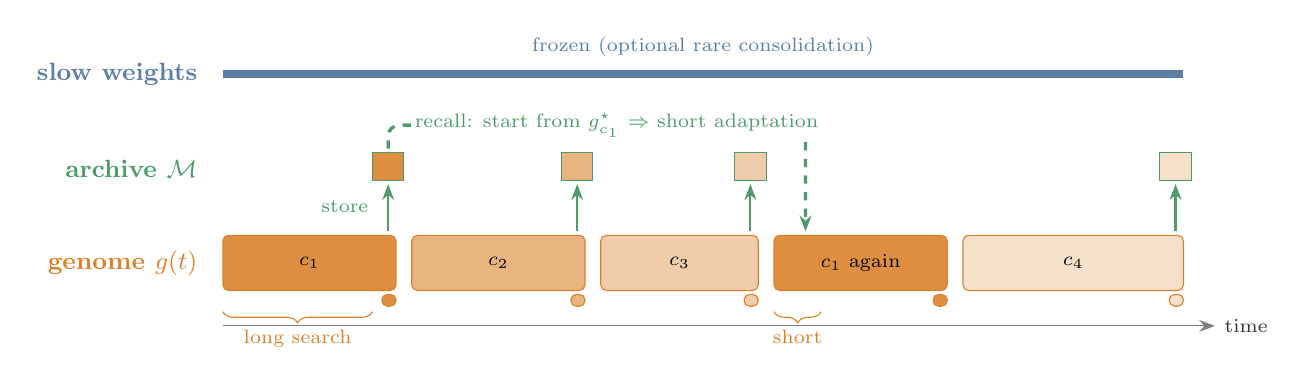
\begin{tikzpicture}[font=\small,>={Stealth[length=2mm]}]
% lanes
\node[anchor=east,text=slow,font=\small\bfseries] at (-0.2,2.4) {slow weights};
\node[anchor=east,text=mem,font=\small\bfseries] at (-0.2,1.2) {archive $\Arch$};
\node[anchor=east,text=fast,font=\small\bfseries] at (-0.2,0) {genome $g(t)$};
\draw[->,gray] (0,-0.8) -- (12.6,-0.8) node[right,font=\scriptsize,text=ink]{time};
% slow lane
\draw[slow,line width=3pt] (0,2.4) -- (12.2,2.4);
\node[font=\scriptsize,text=slow,above] at (6.1,2.5) {frozen (optional rare consolidation)};
% contexts
\foreach \x/\w/\lab/\col in {0/2.2/c_1/fast!90,2.4/2.2/c_2/fast!60,4.8/2.0/c_3/fast!40,7.0/2.2/{c_1\text{ again}}/fast!90,9.4/2.8/c_4/fast!25}{
  \draw[fill=\col,draw=fast,rounded corners=2pt] (\x,-0.35) rectangle (\x+\w,0.35);
  \node[font=\scriptsize] at (\x+\w/2,0) {$\lab$};
  \draw[fill=\col,draw=fast,rounded corners=2pt] (\x+\w-0.18,-0.55) rectangle (\x+\w,-0.4);
}
% stores
\foreach \x/\col in {2.2/fast!90,4.6/fast!60,6.8/fast!40,12.2/fast!25}{
  \draw[->,mem,thick] (\x-0.1,0.4) -- (\x-0.1,1.0);
  \draw[fill=\col,draw=mem] (\x-0.3,1.05) rectangle (\x+0.1,1.4);
}
\node[font=\scriptsize,text=mem] at (1.55,0.72) {store};
% recall arrow
\draw[->,mem,very thick,dashed,rounded corners=4pt] (2.1,1.45) -- (2.1,1.75) -- (7.4,1.75) -- (7.4,0.4);
\node[font=\scriptsize,text=mem,fill=white,inner sep=1pt] at (5.0,1.75) {recall: start from $g^\star_{c_1}$ $\Rightarrow$ short adaptation};
% adaptation speed annotation
\draw[decorate,decoration={brace,amplitude=4pt,mirror,raise=2pt},fast] (0,-0.55) -- (1.9,-0.55) node[midway,below=5pt,font=\scriptsize,text=fast]{long search};
\draw[decorate,decoration={brace,amplitude=4pt,mirror,raise=2pt},fast] (7.0,-0.55) -- (7.6,-0.55) node[midway,below=5pt,font=\scriptsize,text=fast]{short};
\end{tikzpicture}
\caption{\textbf{Three time scales.} The slow weights never change. Each context is solved by a fast search of the genome; its result is stored in the archive. When a context recurs (or a similar one arrives), search starts from the recalled genome and is short.}
\label{fig:timescales}
\end{figure}

% =====================================================================
\section{Discrete genomes and runtime theory}
\label{sec:theory}
% =====================================================================

A discrete late layer (e.g.\ ternary threshold units, F3) makes the genome a string over a finite alphabet, which is exactly the object that EA runtime analysis studies. This section collects what transfers.

\subsection{Re-optimisation after a small change}

Let $\Gen=\Sigma^n$ with $|\Sigma|=s$, and let $g^\star$ be a unique optimum. Call $F$ \emph{OneMax-like} if $F(g) = -\,\big|\{j : g_j \neq g^\star_j\}\big|$, i.e.\ every wrong position costs the same and positions do not interact.

\begin{proposition}[Re-optimisation time from Hamming distance $k$]
\label{prop:reopt}
The (1+1) EA with per-position mutation probability $1/n$ (to a uniformly random other symbol), started at Hamming distance $k$ from $g^\star$ on a OneMax-like $F$, has expected optimisation time
\[
\E[T_k] \;\le\; (s-1)\,e\,n\,H_k \;=\; O(n\log k), \qquad H_k = \textstyle\sum_{i=1}^k \tfrac1i .
\]
\end{proposition}
\begin{proof}
Fitness-level argument. At distance $i$, there are $i$ wrong positions. An improvement occurs if exactly one of them is mutated, to the correct symbol, and nothing else changes; this has probability at least $i\cdot\frac1n\cdot\frac{1}{s-1}\cdot(1-\frac1n)^{n-1}\ge \frac{i}{(s-1)en}$. Elitism means the distance never increases, so the expected time to leave distance $i$ is at most $\frac{(s-1)en}{i}$; summing over $i=1..k$ gives the bound.
\end{proof}

\begin{remark}
A standard coupon-collector argument (each of the $k$ wrong positions must be touched at least once) gives a matching $\Omega(n\log k)$ lower bound for $k$ not too small. The message for continual learning is that \emph{re-adaptation time scales with the size of the change, $\log k$, not with the size of the model}. For general linear functions $F(g)=\sum_j w_j\ind{g_j=g^\star_j}$, tight $O(n\log n)$ bounds from arbitrary initialisation are classical; a clean distance-$k$ bound for arbitrary positive weights is, as far as we know, not standard and is an open question within this project.
\end{remark}

\subsection{How far is reality from OneMax? Measuring epistasis}

Real fitness functions (accuracy of threshold units, routing accuracy) are not linear. Define, at a solution $g$ and for single-position changes $\delta_i,\delta_j$,
\begin{equation}
\Delta^1_i F(g) = F(g\oplus\delta_i) - F(g), \qquad
\Delta^2_{ij} F(g) = F(g\oplus\delta_i\oplus\delta_j) - F(g\oplus\delta_i) - F(g\oplus\delta_j) + F(g),
\end{equation}
and the \emph{relative epistasis} $\varepsilon(g) = \E_{i\ne j}|\Delta^2_{ij}F(g)|\,/\,\E_i|\Delta^1_iF(g)|$. $\varepsilon = 0$ is the additive (OneMax/linear) case where \cref{prop:reopt} applies. On cached features the fitness is deterministic, so $\varepsilon$ can be measured exactly and cheaply.

\subsection{A caveat that sharpens the question}

For a single threshold unit $h(z)=\ind{\ip{w}{z}>\tau}$ with targets $t_b\in\{0,1\}$, the margin surrogate $M(w) = \sum_b (2t_b-1)\ip{w}{z_b} = \ip{w}{v}$, with $v = \sum_b(2t_b-1)z_b$, is linear and is maximised \emph{in closed form} under a sparsity budget by keeping the largest $|v_j|$ with $w_j = \mathrm{sign}(v_j)$. No EA is needed for it. Any value an EA adds must therefore come from the non-linear part of the true objective (thresholding, class imbalance, feature interactions), which is exactly what $\varepsilon$ quantifies.

% =====================================================================
\section{The design space}
\label{sec:design}
% =====================================================================

Every instantiation is a point in a six-dimensional design space:

\begin{center}
\small
\begin{tabularx}{\linewidth}{@{}lX@{}}
\toprule
axis & options \\
\midrule
\textbf{Where} ($\rho$) & input side (prompts) \;/\; all layers \;/\; \textbf{last layers} \;/\; head only \\
\textbf{What} ($A_g$) & routing \;/\; mixing \;/\; masking \;/\; firing \;/\; selection \;/\; learning rule \\
\textbf{Alphabet} & continuous \;/\; binary \;/\; ternary \;/\; categorical (which expert, which path) \\
\textbf{Search} & CMA-ES \;/\; low-rank ES \;/\; GA \;/\; EDA (PBIL, cGA) \;/\; QD (MAP-Elites) \\
\textbf{Fitness} & likelihood \;/\; accuracy, exact match \;/\; worst-group \;/\; return \;/\; lifetime (prequential) \\
\textbf{Memory} & none \;/\; archive keyed by features \;/\; archive keyed by behaviour \;/\; evolved rule (implicit) \\
\bottomrule
\end{tabularx}
\end{center}

Two further choices concern the \emph{slow} side: whether the library is built for \emph{diversity} (F2, F4) and whether the slow system is ever \emph{consolidated} from frequently used genomes (distilling a genome into the backbone or spawning a new expert). The latter is the natural long-term outer loop and is out of scope here.

% =====================================================================
\section{Five instantiations}
\label{sec:instances}
% =====================================================================

Each instantiation has a self-contained proposal (\texttt{research/proposals/F-late-ea/F*.md}) with the full benchmark protocol. Here we give the idea and its central equation in the notation above.

\subsection*{F1 --- EvoRouter: evolved routing in a pretrained mixture-of-experts}
A pretrained MoE language model is frozen. In the last $L'$ MoE layers the router logits are shifted by a genome, and top-$k$ expert selection is kept \emph{hard}:
\begin{equation}
\tilde s_\ell(h,x) = W_\ell h + b_\ell + U_\ell P\,\bar e(x),\qquad \ell > L-L',\qquad g = (b_\ell, U_\ell)_\ell,\ n = KL'(1+d').
\end{equation}
Top-$k$ has no useful gradient; the EA optimises the deployed discrete routing directly. Multiple-choice scoring is compute-separable with $\rho = L'/L$, and one genome per domain is archived.

\subsection*{F2 --- EvoCompose: composition of a diversified expert library}
A library of $K$ adapters is trained to be \emph{expert} in-domain and \emph{diverse} where the ensemble is uncertain:
\begin{equation}
\mathcal{L}_k = \E_{\Dist_k}\big[-\log p_k(y\mid x)\big] - \lambda\,\E_{x\sim\Dist_{\text{pool}}}\Big[(1-a(x))\tfrac{1}{K-1}\textstyle\sum_{j\neq k}\omega_{kj}(x)\,\JS\big(p_k(\cdot\mid x)\,\|\,\sg[p_j(\cdot\mid x)]\big)\Big],
\end{equation}
with agreeableness $a(x)$ (e.g.\ the best expert's confidence in the true label) and an expertness weight $\omega_{kj}$. Per task, a genome of mixing coefficients composes the library only in the last layers:
\begin{equation}
W'_\ell = W_\ell + \textstyle\sum_{k=1}^K \alpha_{\gamma(\ell),k}\,B_{\ell,k}A_{\ell,k},\qquad g = (\alpha_{\gamma,k}) \in\R^{G\times K}.
\end{equation}

\subsection*{F3 --- The Sandwich: frozen encoder, evolved discrete firing layer, frozen decoder}

\begin{center}
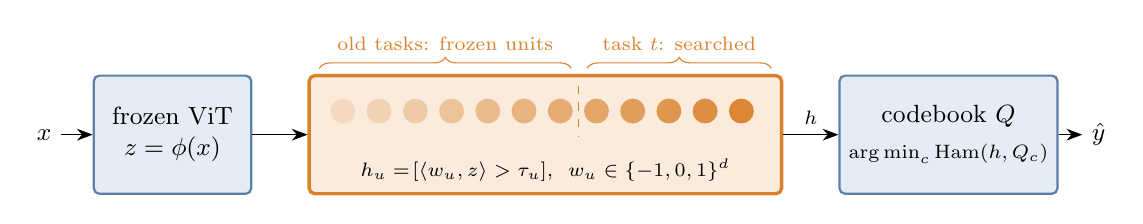
\begin{tikzpicture}[font=\small,>={Stealth[length=2mm]},
  s/.style={draw=slow,fill=slowbg,rounded corners=2pt,thick,minimum height=1.5cm,align=center},
  f/.style={draw=fast,fill=fastbg,rounded corners=2pt,very thick,minimum height=1.5cm,align=center}]
\node (x) {$x$};
\node[s,right=0.4cm of x,minimum width=2.0cm] (enc) {frozen ViT\\ $z=\phi(x)$};
\node[f,right=0.7cm of enc,minimum width=6.0cm] (units) {};
\foreach \i in {0,...,11}{ \fill[fast!\the\numexpr 30+6*\i\relax] ($(units.west)+(0.45+0.46*\i,0.3)$) circle (4.5pt); }
\draw[fast,dashed] ($(units.west)+(3.44,0.62)$) -- ($(units.west)+(3.44,-0.02)$);
\node[font=\scriptsize,anchor=south] at ($(units.south)+(0,0.05)$) {$h_u=\ind{\ip{w_u}{z}>\tau_u}$,\ \ $w_u\in\{-1,0,1\}^d$};
\node[s,right=0.7cm of units,minimum width=2.4cm] (dec) {codebook $Q$\\[2pt] {\scriptsize $\argmin_c \Ham(h,Q_c)$}};
\node[right=0.3cm of dec] (y) {$\hat y$};
\draw[->] (x)--(enc); \draw[->] (enc)--(units); \draw[->] (units)--node[above,font=\scriptsize]{$h$}(dec); \draw[->] (dec)--(y);
\draw[decorate,decoration={brace,amplitude=4pt,raise=2pt},fast] ($(units.north west)+(0.15,0)$) -- ($(units.north west)+(3.35,0)$) node[midway,above=5pt,font=\scriptsize,text=fast]{old tasks: frozen units};
\draw[decorate,decoration={brace,amplitude=4pt,raise=2pt},fast] ($(units.north west)+(3.55,0)$) -- ($(units.north east)+(-0.15,0)$) node[midway,above=5pt,font=\scriptsize,text=fast]{task $t$: searched};
\end{tikzpicture}
\end{center}

Units decompose: for fixed codewords each unit $u$ has target bits $t_{b,u} = Q_{y_b,u}$ and an independent fitness
\begin{equation}
F_u(w_u) = \tfrac1B\textstyle\sum_b \ind{\ind{\ip{w_u}{z_b}>\tau_u} = t_{b,u}},
\end{equation}
so $m$ searches run in parallel on cached features at $10^4$--$10^6$ evaluations per second, with $\tau_u$ set optimally by one sort. New tasks add units; old units never change. This is the natural test-bed for \cref{prop:reopt} and the epistasis measure $\varepsilon$.

\subsection*{F4 --- Repertoire adaptation inside a learned model}
Offline, MAP-Elites builds a repertoire $\{(\pi_j, d_j, f_j)\}$ of diverse skills. After a change (e.g.\ robot damage) a small genome blends skills near a target descriptor and adds feedback,
\begin{equation}
\pi_g(s) = \textstyle\sum_{j\in\mathcal{N}_q(d^\star)} w_j(g)\,\pi_j(s) + K_\kappa\,\phi_{\text{fb}}(s),\qquad g = (d^\star,\log T,\kappa),
\end{equation}
and CMA-ES evaluates the population inside a learned residual model $\hat s_{t+1} = \mathrm{Sim}(s_t,a_t) + \delta_\omega(s_t,a_t)$, with a pessimistic fitness $\hat F(g) = \mathrm{mean}_e R_e(g) - \beta\,\mathrm{std}_e R_e(g)$ over an ensemble. The population lives in the model; the real system only sees the champion.

\subsection*{F5 --- Evolved plasticity}
The EA moves one level up and searches the parameters $\theta$ of a local learning rule for the late layer,
\begin{equation}
\Delta W_t = \eta\odot\Big[M_t\big(A\odot o_tz_t^\top + B\odot o_t\mathbf 1^\top + C\odot \mathbf 1 z_t^\top + D\big) + E\odot e_tz_t^\top\Big] - \lambda\odot W_t,
\end{equation}
optimising the prequential lifetime objective $\E_{c}\big[\frac{1}{T}\sum_t \mathrm{perf}(\hat y_t,y_t)\big]$ over a distribution of drifting contexts. The error term $E\odot e_tz_t^\top$ makes online SGD a member of the family, so an evolved rule must beat it to matter.

\subsection*{At a glance}
\begin{center}
\small
\begin{tabularx}{\linewidth}{@{}lL{3.4cm}L{2.2cm}L{3.3cm}Y@{}}
\toprule
 & genome & $n$ & separability & EA-specific advantage \\
\midrule
F1 & router biases (+ conditioning) & $10^2$--$10^4$ & compute ($\rho=L'/L$) & hard top-$k$ routing \\
F2 & mixing coefficients & $10^1$--$10^3$ & compute (late layers) & multi-modal mixing; population $=$ ensemble \\
F3 & ternary unit weights & $10^4$--$10^5$ trits & compute ($\rho\approx0$) & discrete; theory; massive throughput \\
F4 & descriptor target, blend, gains & $10^1$--$10^2$ & memory only; parallel in model & noisy, multi-modal model fitness \\
F5 & rule parameters & $10^1$--$10^4$ & compute over contexts & long, non-differentiable lifetimes \\
\bottomrule
\end{tabularx}
\end{center}

% =====================================================================
\section{Related work}
\label{sec:related}
% =====================================================================

\paragraph{Evolution strategies at scale.}
ES as a scalable alternative to RL \cite{salimans2017es} and deep neuroevolution with GAs \cite{such2017deep} showed that population methods can train deep networks given enough parallel compute. EGGROLL \cite{eggroll} makes ES on billion-parameter models practical through low-rank perturbations, and ES has been shown competitive with RL for LLM fine-tuning \cite{qiu2025esscale}, with the caveat that its dense, high-norm updates can cause forgetting \cite{esforgetting}. These are the ``deep'' end of \cref{fig:design-space}; this document argues for the ``shallow and late'' end. CMA-ES \cite{hansen2016cma}, natural evolution strategies \cite{wierstra2014nes} and IGO \cite{ollivier2017igo} provide the algorithmic backbone.

\paragraph{Frozen features with a small evolved controller.}
World Models \cite{ha2018world} trains a VAE and a recurrent model by gradients and then evolves an 867-parameter controller with CMA-ES --- the clearest precedent for the slow/fast split. PathNet \cite{fernando2017pathnet} uses a GA to select paths through layers of modules and freezes the paths of earlier tasks, an early instance of evolved, memory-backed continual learning.

\paragraph{Low-dimensional, gradient-free adaptation.}
Fine-tuning has a small intrinsic dimension \cite{li2018intrinsic,aghajanyan2021intrinsic}. Black-box tuning optimises a low-dimensional prompt projection with CMA-ES \cite{sun2022bbt}. FOA adapts a frozen vision transformer at test time with CMA-ES on input prompts, using forward passes only \cite{niu2024foa}.

\paragraph{Composing and merging experts.}
Task arithmetic \cite{ilharco2023task} and learned merging coefficients \cite{yang2024adamerging} show that fine-tuned deltas compose. LoraHub \cite{huang2024lorahub} searches LoRA mixing weights gradient-free from a few examples; Transformer$^2$ \cite{sun2025transformer2} mixes singular-value expert vectors at test time, including by CEM. Evolutionary model merging \cite{akiba2025evomerge}, CycleQD \cite{kuroki2025cycleqd} and M2N2 \cite{abrantes2025m2n2} evolve merge recipes and maintain diversity through QD or resource competition. Libraries of domain experts can be built by branching and training separately \cite{li2022btm,sukhbaatar2024btx} and routed without search \cite{ostapenko2024arrow}. Methods that train models to disagree out of distribution \cite{lee2023divdis,pagliardini2023dbat} and population-level diversity objectives \cite{parkerholder2020dvd} motivate the diversity-regularised library of F2.

\paragraph{Mixture-of-experts routing.}
C3PO \cite{li2025c3po} re-mixes expert weights in the last layers of pretrained MoE models at test time using neighbour-based surrogates and recovers a large part of an oracle routing gap. Evolutionary expert pruning \cite{liu2024eep} and auxiliary-loss-free bias-based load balancing \cite{wang2024auxfree} show, respectively, that EAs apply to MoE structure and that per-expert biases are a meaningful low-dimensional control. OLMoE \cite{muennighoff2024olmoe} is a fully open testbed.

\paragraph{Discrete computation and masks.}
Binary masks over fixed random weights (supermasks) reach good accuracy \cite{zhou2019deconstructing,ramanujan2020hidden}, and one mask per task yields continual learning without forgetting \cite{wortsman2020supsup,masana2021ternary}. Weight-agnostic networks \cite{gaier2019wann}, Tsetlin machines \cite{granmo2018tsetlin}, logic-gate networks \cite{petersen2022logic} and ternary LLMs \cite{ma2024bitnet} show that discrete computation is viable. Frozen pretrained features with simple heads are strong continual learners \cite{zhou2023revisiting,mcdonnell2023ranpac,wang2022l2p}, and last-layer retraining is sufficient for robustness to spurious correlations \cite{kirichenko2023dfr}.

\paragraph{Fast adaptation from a repertoire.}
Intelligent Trial and Error \cite{cully2015robots} builds a MAP-Elites \cite{mouret2015mapelites} repertoire offline and adapts to damage online with Bayesian optimisation over it; follow-ups add reset-free operation \cite{chatzilygeroudis2018rte} and selection among repertoires \cite{kaushik2020aprol}. Black-DROPS \cite{chatzilygeroudis2017blackdrops} runs CMA-ES inside learned dynamics models. QDax \cite{lim2023accelerated,chalumeau2024qdax} makes QD massively parallel on accelerators.

\paragraph{Evolved plasticity and meta-learning.}
Evolved Hebbian rules let randomly initialised networks self-organise within an episode and cope with unseen damage \cite{najarro2020hebbian}; differentiable plasticity and neuromodulation \cite{miconi2018differentiable,miconi2019backpropamine} and fast weights \cite{ba2016fastweights} are the gradient-based counterparts. Context-vector meta-learning \cite{zintgraf2019cavia} and ES-based MAML \cite{song2020esmaml} adapt only a small set of parameters.

\paragraph{Runtime theory.}
The (1+1) EA optimises linear functions in $\Theta(n\log n)$ \cite{droste2002linear,witt2013tight}; dynamic and re-optimisation settings have been analysed for OneMax variants \cite{kotzing2015dynamic} and linear functions under dynamic constraints \cite{shi2019reopt}. \Cref{sec:theory} asks how far these results carry to a discrete late layer.

\paragraph{Gap.}
Existing work either (i)~evolves a small late component \emph{once} (merging recipes, controllers), (ii)~adapts at test time \emph{without memory} (FOA, C3PO, Transformer$^2$), or (iii)~learns continually with \emph{gradient}-found masks or prompts (SupSup, L2P). The combination studied here --- a frozen or diversified library, a late and separable evolved layer exploiting massive parallelism, and an archive of genomes as memory, evaluated on adaptation speed and forgetting --- is, to our knowledge, open.

% =====================================================================
\section{Open questions}
\label{sec:open}
% =====================================================================
\begin{enumerate}
\item \textbf{Where is the cut?} How small can $\rho$ be before the frozen components cap what adaptation can reach? Is there a principled way to choose $\ell$ (e.g.\ from layer-wise task specificity)?
\item \textbf{Diversity of the slow system.} Does a library trained for diversity make the fast search easier? Can this be quantified, e.g.\ via the effective rank of per-example correctness vectors across experts?
\item \textbf{Keys and recall.} Which context keys make recall reliable? When does soft blending of archived genomes beat hard recall?
\item \textbf{Theory beyond OneMax.} Distance-$k$ re-optimisation bounds for general linear functions; bounds in terms of measured epistasis $\varepsilon$.
\item \textbf{Consolidation.} When and how should frequently recalled genomes be distilled into the slow system, and does that re-introduce forgetting?
\item \textbf{Search at deployment vs.\ learned learning.} When does an evolved rule (F5) replace search plus archive (F1--F4), and can they be combined hierarchically?
\end{enumerate}

% =====================================================================
\begin{thebibliography}{99}\small
\bibitem{abrantes2025m2n2} J.~Abrantes, R.~Lange, Y.~Tang. Competition and attraction improve model fusion (M2N2). GECCO 2025. arXiv:2508.16204.
\bibitem{aghajanyan2021intrinsic} A.~Aghajanyan, L.~Zettlemoyer, S.~Gupta. Intrinsic dimensionality explains the effectiveness of language model fine-tuning. ACL 2021. arXiv:2012.13255.
\bibitem{akiba2025evomerge} T.~Akiba, M.~Shing, Y.~Tang, Q.~Sun, D.~Ha. Evolutionary optimization of model merging recipes. Nature Machine Intelligence 2025. arXiv:2403.13187.
\bibitem{ba2016fastweights} J.~Ba, G.~Hinton, V.~Mnih, J.~Leibo, C.~Ionescu. Using fast weights to attend to the recent past. NeurIPS 2016. arXiv:1610.06258.
\bibitem{chalumeau2024qdax} F.~Chalumeau et al. QDax: a library for quality-diversity and population-based algorithms with hardware acceleration. JMLR 2024. arXiv:2308.03665.
\bibitem{chatzilygeroudis2017blackdrops} K.~Chatzilygeroudis, R.~Rama, R.~Kaushik, D.~Goepp, V.~Vassiliades, J.-B.~Mouret. Black-box data-efficient policy search for robotics. IROS 2017. arXiv:1703.07261.
\bibitem{chatzilygeroudis2018rte} K.~Chatzilygeroudis, V.~Vassiliades, J.-B.~Mouret. Reset-free trial-and-error learning for robot damage recovery. Robotics and Autonomous Systems 2018. arXiv:1610.04213.
\bibitem{cully2015robots} A.~Cully, J.~Clune, D.~Tarapore, J.-B.~Mouret. Robots that can adapt like animals. Nature 521, 2015. arXiv:1407.3501.
\bibitem{droste2002linear} S.~Droste, T.~Jansen, I.~Wegener. On the analysis of the (1+1) evolutionary algorithm. Theoretical Computer Science 276, 2002.
\bibitem{eggroll} Evolution strategies at the hyperscale (EGGROLL). arXiv:2511.16652, 2025.
\bibitem{esforgetting} Evolutionary strategies lead to catastrophic forgetting in LLMs. arXiv:2601.20861, 2026.
\bibitem{fernando2017pathnet} C.~Fernando et al. PathNet: evolution channels gradient descent in super neural networks. arXiv:1701.08734, 2017.
\bibitem{gaier2019wann} A.~Gaier, D.~Ha. Weight agnostic neural networks. NeurIPS 2019. arXiv:1906.04358.
\bibitem{granmo2018tsetlin} O.-C.~Granmo. The Tsetlin machine. arXiv:1804.01508, 2018.
\bibitem{ha2018world} D.~Ha, J.~Schmidhuber. World models / Recurrent world models facilitate policy evolution. NeurIPS 2018. arXiv:1803.10122.
\bibitem{hansen2016cma} N.~Hansen. The CMA evolution strategy: a tutorial. arXiv:1604.00772, 2016.
\bibitem{huang2024lorahub} C.~Huang, Q.~Liu, B.~Y.~Lin, T.~Pang, C.~Du, M.~Lin. LoraHub: efficient cross-task generalization via dynamic LoRA composition. COLM 2024. arXiv:2307.13269.
\bibitem{ilharco2023task} G.~Ilharco et al. Editing models with task arithmetic. ICLR 2023. arXiv:2212.04089.
\bibitem{kaushik2020aprol} R.~Kaushik, P.~Desreumaux, J.-B.~Mouret. Adaptive prior selection for repertoire-based online adaptation in robotics. Frontiers in Robotics and AI 2020. arXiv:1907.07029.
\bibitem{kirichenko2023dfr} P.~Kirichenko, P.~Izmailov, A.~G.~Wilson. Last layer re-training is sufficient for robustness to spurious correlations. ICLR 2023. arXiv:2204.02937.
\bibitem{kotzing2015dynamic} T.~Kötzing, A.~Lissovoi, C.~Witt. (1+1) EA on generalized dynamic OneMax. FOGA 2015.
\bibitem{kuroki2025cycleqd} S.~Kuroki, T.~Nakamura, T.~Akiba, Y.~Tang. Agent skill acquisition for LLMs via CycleQD. ICLR 2025. arXiv:2410.14735.
\bibitem{lee2023divdis} Y.~Lee, H.~Yao, C.~Finn. Diversify and disambiguate: learning from underspecified data. ICLR 2023. arXiv:2202.03418.
\bibitem{li2018intrinsic} C.~Li, H.~Farkhoor, R.~Liu, J.~Yosinski. Measuring the intrinsic dimension of objective landscapes. ICLR 2018. arXiv:1804.08838.
\bibitem{li2022btm} M.~Li et al. Branch-train-merge: embarrassingly parallel training of expert language models. arXiv:2208.03306, 2022.
\bibitem{li2025c3po} Z.~Li, Z.~Li, T.~Zhou. C3PO: critical-layer, core-expert, collaborative pathway optimization for test-time expert re-mixing. arXiv:2504.07964, 2025.
\bibitem{lim2023accelerated} B.~Lim, M.~Allard, L.~Grillotti, A.~Cully. Accelerated quality-diversity through massive parallelism. TMLR 2023. arXiv:2202.01258.
\bibitem{liu2024eep} E.~Liu et al. Efficient expert pruning for sparse mixture-of-experts language models (EEP). arXiv:2407.00945, 2024.
\bibitem{ma2024bitnet} S.~Ma et al. The era of 1-bit LLMs: all large language models are in 1.58 bits. arXiv:2402.17764, 2024.
\bibitem{masana2021ternary} M.~Masana, T.~Tuytelaars, J.~van de Weijer. Ternary feature masks: zero-forgetting for task-incremental learning. CVPR Workshops 2021. arXiv:2001.08714.
\bibitem{mcdonnell2023ranpac} M.~D.~McDonnell, D.~Gong, A.~Parvaneh, E.~Abbasnejad, A.~van den Hengel. RanPAC: random projections and pre-trained models for continual learning. NeurIPS 2023. arXiv:2307.02251.
\bibitem{miconi2018differentiable} T.~Miconi, J.~Clune, K.~O.~Stanley. Differentiable plasticity. ICML 2018. arXiv:1804.02464.
\bibitem{miconi2019backpropamine} T.~Miconi, A.~Rawal, J.~Clune, K.~O.~Stanley. Backpropamine: training self-modifying neural networks with differentiable neuromodulated plasticity. ICLR 2019. arXiv:2002.10585.
\bibitem{mouret2015mapelites} J.-B.~Mouret, J.~Clune. Illuminating search spaces by mapping elites. arXiv:1504.04909, 2015.
\bibitem{muennighoff2024olmoe} N.~Muennighoff et al. OLMoE: open mixture-of-experts language models. arXiv:2409.02060, 2024.
\bibitem{najarro2020hebbian} E.~Najarro, S.~Risi. Meta-learning through Hebbian plasticity in random networks. NeurIPS 2020. arXiv:2007.02686.
\bibitem{niu2024foa} S.~Niu, C.~Miao, G.~Chen, P.~Wu, P.~Zhao. Test-time model adaptation with only forward passes. ICML 2024. arXiv:2404.01650.
\bibitem{ollivier2017igo} Y.~Ollivier, L.~Arnold, A.~Auger, N.~Hansen. Information-geometric optimization algorithms: a unifying picture via invariance principles. JMLR 2017. arXiv:1106.3708.
\bibitem{ostapenko2024arrow} O.~Ostapenko et al. Towards modular LLMs by building and reusing a library of LoRAs. ICML 2024. arXiv:2405.11157.
\bibitem{pagliardini2023dbat} M.~Pagliardini, M.~Jaggi, F.~Fleuret, S.~P.~Karimireddy. Agree to disagree: diversity through disagreement for better transferability. ICLR 2023. arXiv:2202.04414.
\bibitem{parkerholder2020dvd} J.~Parker-Holder, A.~Pacchiano, K.~Choromanski, S.~Roberts. Effective diversity in population-based reinforcement learning. NeurIPS 2020. arXiv:2002.00632.
\bibitem{petersen2022logic} F.~Petersen, C.~Borgelt, H.~Kuehne, O.~Deussen. Deep differentiable logic gate networks. NeurIPS 2022. arXiv:2210.08277.
\bibitem{qiu2025esscale} X.~Qiu et al. Evolution strategies at scale: LLM fine-tuning beyond reinforcement learning. arXiv:2509.24372, 2025.
\bibitem{ramanujan2020hidden} V.~Ramanujan, M.~Wortsman, A.~Kembhavi, A.~Farhadi, M.~Rastegari. What's hidden in a randomly weighted neural network? CVPR 2020. arXiv:1911.13299.
\bibitem{salimans2017es} T.~Salimans, J.~Ho, X.~Chen, S.~Sidor, I.~Sutskever. Evolution strategies as a scalable alternative to reinforcement learning. arXiv:1703.03864, 2017.
\bibitem{shi2019reopt} F.~Shi, M.~Schirneck, T.~Friedrich, T.~Kötzing, F.~Neumann. Reoptimization time analysis of evolutionary algorithms on linear functions under dynamic uniform constraints. Algorithmica 81, 2019.
\bibitem{song2020esmaml} X.~Song et al. ES-MAML: simple Hessian-free meta learning. ICLR 2020. arXiv:1910.01215.
\bibitem{such2017deep} F.~P.~Such et al. Deep neuroevolution: genetic algorithms are a competitive alternative for training deep neural networks for reinforcement learning. arXiv:1712.06567, 2017.
\bibitem{sukhbaatar2024btx} S.~Sukhbaatar et al. Branch-train-MiX: mixing expert LLMs into a mixture-of-experts LLM. arXiv:2403.07816, 2024.
\bibitem{sun2022bbt} T.~Sun, Y.~Shao, H.~Qian, X.~Huang, X.~Qiu. Black-box tuning for language-model-as-a-service. ICML 2022. arXiv:2201.03514.
\bibitem{sun2025transformer2} Q.~Sun, E.~Cetin, Y.~Tang. Transformer$^2$: self-adaptive LLMs. ICLR 2025. arXiv:2501.06252.
\bibitem{wang2022l2p} Z.~Wang et al. Learning to prompt for continual learning. CVPR 2022. arXiv:2112.08654.
\bibitem{wang2024auxfree} L.~Wang, H.~Gao, C.~Zhao, X.~Sun, D.~Dai. Auxiliary-loss-free load balancing strategy for mixture-of-experts. arXiv:2408.15664, 2024.
\bibitem{wierstra2014nes} D.~Wierstra, T.~Schaul, T.~Glasmachers, Y.~Sun, J.~Peters, J.~Schmidhuber. Natural evolution strategies. JMLR 2014. arXiv:1106.4487.
\bibitem{witt2013tight} C.~Witt. Tight bounds on the optimization time of a randomized search heuristic on linear functions. Combinatorics, Probability and Computing 22, 2013.
\bibitem{wortsman2020supsup} M.~Wortsman et al. Supermasks in superposition. NeurIPS 2020. arXiv:2006.14769.
\bibitem{yang2024adamerging} E.~Yang et al. AdaMerging: adaptive model merging for multi-task learning. ICLR 2024. arXiv:2310.02575.
\bibitem{zhou2019deconstructing} H.~Zhou, J.~Lan, R.~Liu, J.~Yosinski. Deconstructing lottery tickets: zeros, signs, and the supermask. NeurIPS 2019. arXiv:1905.01067.
\bibitem{zhou2023revisiting} D.-W.~Zhou, Z.-W.~Cai, H.-J.~Ye, D.-C.~Zhan, Z.~Liu. Revisiting class-incremental learning with pre-trained models: generalizability and adaptivity are all you need. IJCV 2024. arXiv:2303.07338.
\bibitem{zintgraf2019cavia} L.~Zintgraf, K.~Shiarlis, V.~Kurin, K.~Hofmann, S.~Whiteson. Fast context adaptation via meta-learning (CAVIA). ICML 2019. arXiv:1810.03642.
\end{thebibliography}

\end{document}
